			
\section{Communications Mobiles}
	\subsection{GSM (2G)}
		Se base sur un systheme de cellules haxagonales de taille différente
		\begin{itemize}
			\item Macrocell (30km)
			\item Microcell (2-4km)
			\item Picocell (200m)
			\item Femtocell
		\end{itemize}
		
		Une tour associé a chaque cellules, les \textbf{BTS}(Base Transceiver Station). Ces tours sont associées en groupes a une station, les \textbf{BSC} (Base station controller). Enfin les BSC sont associé a un centre \textbf{MSC} (Mobile service switching center). Ces centre sont relié par 3G a internet.
		
		Les utilisateur communique avec les BTS.
		
	\subsection{Réutilisation des fréquences}
			On fixe un niveau admissible d'interférence entre les différents tours (elle utilise la meme fréquence), souvent a 10db. Il font donc réfléchir au placement des tours.
			\begin{figure}[H]
				\centering
				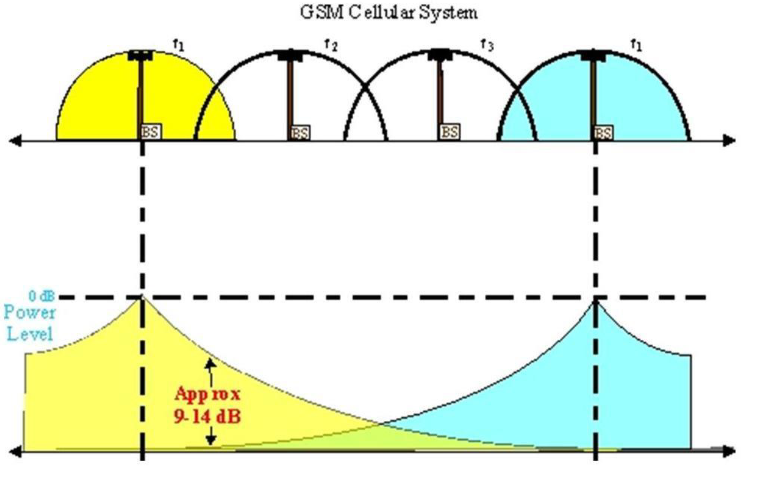
\includegraphics[width=0.7\textwidth]{img/CM/RF.png}
			\end{figure}
			
			On va utiliser un \textbf{Planning de fréquences}, qui va essayer de distribuer les fréquences entre les tours pour eviter au max les interférences.
 
 			\begin{figure}[H]
				\centering
				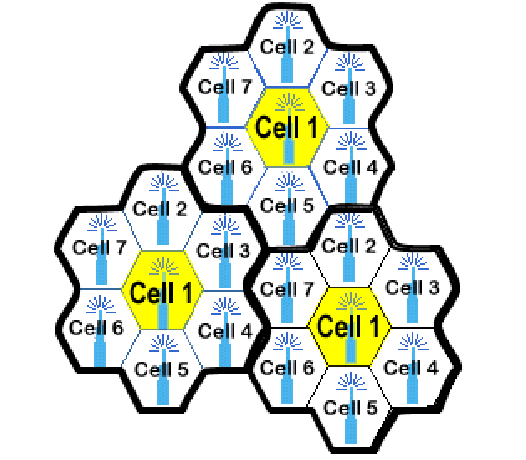
\includegraphics[width=0.5\textwidth]{img/CM/PF.png}
			\end{figure}
			
			Les bandes fréquences GSM \textbf{Montantes} (Envois donnée vers stations) est de 890 à 915 MHz et descendantes (Stations envoi donnée a user) 935 à 960 MHz
			
	\subsection{Modulations}
		GSM utilie \textbf{GMSK} (Gaussian minimum shift keying) pour l'envoi des données numérique la largueur de bande est de 200 kHz. Tres robuste mais peu efficace
		
	\subsection{Multiplexage}
 		Couplage du TDMA et du FDMA ( cf section Transmission des données)
 		
 		Chaque tour founit 8 timeslot et 124 cannaux de 200kHz. Deux utilisateurs peuvent partager un timeslots (\textbf{Half rate}, chacun son tour). Petit décalage entres les timesolts déscendant et montant.
 		
 		\begin{figure}[H]
 			\centering
 			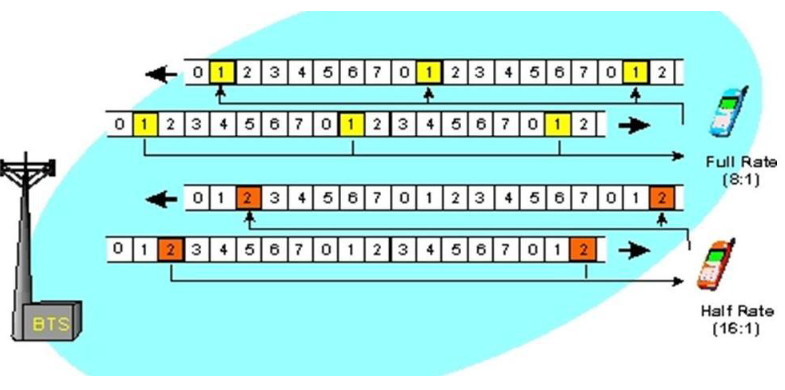
\includegraphics[width=\textwidth]{img/CM/HR.png}
 		\end{figure}
 		
 		\subsubsection{Structure timeslot}
 			5 types de paquets (\textbf{burst}), l'emission d'un paquet  correspond a l'emission de 156.25 bits:
 			
 			\begin{itemize}
 				\item \textbf{Acces} : demande de contact avec le réseau
 				\item \textbf{Synchronisation} : Localisation + réception d'un fréquence pour communiquer
 				\item \textbf{Normal} : Envoi du message
 				\item \textbf{Correction fréquence} : Prévention d'interférence possible (burst vide)
 				\item \textbf{Bourrage} : Complete le vide
 			\end{itemize}
 			
 	\subsection{Distorsion}
 		Probleme est la perte du signal entre la tour et l'utilisateur, plusieur raisons
 		\begin{itemize}
 			\item \textbf{Multi-trajet} : Signal prends plusieur chemin pour rejoindre la station a cause des interférence (rebond sur un immeuble)
 			\item \textbf{Shadowing} : Un objet ostrue la transmission
 			\item \textbf{Effet doppler} Décalage de fréquence d’une onde entre l’émission et la réception quand la distance entre les deux varie au cours du temps. Cet effet est causé par le déplacement de l’utilisateur par rapport à l’antenne
 		\end{itemize}
 		
 		Plusieurs solutions :
 		\begin{itemize}
 			\item Codes correcteurs d'erreur
 			\item diversifier les fréquences du signal (Frequency hopping)
 			\item Jouer sur la modulation
 			\item Égalisation du signal
 		\end{itemize}
 		
 		\textbf{Frequency Hopping} : On transmet le premier burst a une fréquence $f_1$, la deuxieme a fréquence $f_2$ et le troisieme a $f_3$ et on réutilise ces fréquence dans cet ordre
 		
 		
 	\subsection{Alignement dynamique}
 		Si 2 utilisateurs utilise des timeslot différents maiq que leur distance a la tour varie, il est pas impossible que les signaux s'interfère.
 		
 		On doit adapter le time slot en fonction du temps que le signal va prendre pour arriver à la tour. Cela revient à ajouter du décalage temporel de façon à ce que la station de base tombe toujours bien sur le timeslot qu’il faut
 		
 		Ne peut se faire que en montant car il peut y avoir plusieur utilisateur. En descendant,  se serait ridicule puisqu’il n’y a qu’un seul destinataire possible. (le GSM ne parle qu’à la station alors que la station parle à beaucoup de GSM)
 		
 	\subsection{Accès au système}
 	
 		La premier connexion a la tour :GSM regarde les canaux libre et parle a la station qui va lui attribuer un canal et timeslots
 		
 		Arrive quand :
 		\begin{itemize}
 			\item premiere connexion
 			\item Pour initier un appel
 			\item Pour répondre a un appel
 			\item Envoyer ou recevoir des données
 		\end{itemize}
 		
 	\subsection{Handover}
 		Quand le GSM change de BTS en brisant l'ancienne et puis crée une nouvelle liaison. A lieu quand  un diminution de la qualitité et donc propose nouvelle BST au GSM (par MSC) 
 		
 	\subsection{Internet sur GSM}
 		\subsubsection{GPRS (2.5G)}
 			Utilise les paquet de transmission pour transmettre internet. On tranmet un paquet que quand necessaire car facturé au volume
 			
 			Debit de 40-100 kb/s
 			
 		\subsubsection{Edge (2.75G)}
 			Modualtion 8-PSK qui permet 3/4 fois plus de débit. Implique du matériél adapté sur les stations et terminaux.
 			
 		\subsubsection{UMTS (3G)}
 			Fréquence 1885-2025 MHz montant 2110-2200 MHz descendant. Compatible mondial. Largueur de bande de 5MHz
 			
 			On utilise W-CDM (Une sorte de CDMA)
 			\begin{itemize}
 				\item Plus d'alignement dynamique nécessaire
 				\item Soft handover possible
 				\item Plus d'interférence
 			\end{itemize}
 			
 			Vitesse :
 			\begin{itemize}
 				\item 2 Mb/s stations fixe (pietons)
 				\item 144 kb/s Sation mobile (en voiture)
 			\end{itemize}
 			
 		\subsubsection{LTE (4G)}
 			Utilise modulation OFDM (descendant) et SC-FDMA (montant). Tres flexible. Utilise des fréquences de 450Mhz a 3.8Ghz selon les pays et modulation adaptative qui permet d'adapter la constellation utilisé. Si la liaison est bonne alors on auraune constellation avec beaucoup de points permettant un meilleur debit. Si mauvaise liaison, constellation avec peut de points pour eviter les erreurs et donc debit plus faible.
 			
 			Différence avec anciens systheme
 			\begin{itemize}
 				\item \textbf{AMC} : \textit{Adaptative Modulation and Coding} : On adapte le débit à la qualité de la transmission. Si on a une transmission de qualité, on va augmenter la taille de la constellation pour augmenter le débit
 				\item \textbf{Multiplexage/modulation} : Modulation OFDM : Consiste à diviser le temps et les fréquences utilisables en un quadrillage où chaque carré représente une ressource. on va alors allouer aux utilisateurs des ressources de manière dynamique (adaptative) en fonction des besoins de l’utilisateur, du trafic, des interférences et/ou de la mobilité de l’utilisateur.
 				\item \textbf{Bande variable} : dû à l’OFDM, on peut utiliser une bande variante pour une transmission donnée. Cela rajoute une complexité au niveau des émetteurs et récepteurs 4G. 
 				\item \textbf{HARQ} : \textit{Hybrid Automatic Repeat reQuest} : Lorsqu’un bloc n’est pas acquitté, on ne retransmet pas toute la frame mais plutôt certains bits.
 			\end{itemize}